\section{Partitioning}
	Il Partitional Clustering scompone un set di dati in un insieme di cluster disgiunti.
	\\[1\baselineskip]
	Dato un set di dati di $n$ punti, un metodo di partizionamento costruisce $k$ ($k \leq n$) partizioni, con ciascuna partizione che rappresenta un cluster; classifica i dati in $k$ gruppi soddisfacendo i seguenti requisiti:
		\begin{enumerate}
			\item ogni gruppo contiene almeno un punto;
			\item ogni punto appartiene esattamente a un gruppo.
		\end{enumerate}
	
	$\textbf{Nota}:$ per il partizionamento Fuzzy (spiegato successivamente), un punto può appartenere a più di un gruppo.
	\\[1\baselineskip]
	Molti algoritmi di clustering partizionale tentano di minimizzare una funzione obiettivo.
	\\
	Ad esempio, in K-Means e K-Medoidi la funzione (nota anche come $\textbf{funzione di distorsione}$) è:
		$$ \sum_{i=1}^{k} \sum_{j=1}^{|C_{i}|} \left[ d(x_{j}, \textrm{center}(i)) \right] $$

	dove $|C_{i}|$ è il numero di punti nel cluster $i$, $d(x_{j}, \textrm{center}(i))$ è la distanza tra il punto $x_{j}$ e il centro $i$, e $k$ è il numero di clusters.

	\clearpage

	\subsection{K-Means}
		Questo algoritmo di clustering opera in maniera molto semplice:
			\begin{enumerate}
				\item sceglie $k$ centri a caso $c_{1}, \ldots, c_{k}$;
				\item dati i nuovi centri $c_1, \ldots, c_k$, minimizza la distanza euclidea $\|p - c_{i}\|^{2}$, ponendo $p$ nel cluster $C_i$ del centro più vicino $c_i$;
					\\[1\baselineskip]
					$\textbf{Reminder}:$ $\|\overrightarrow{u}\|$ è la norma del vettore u, ovvero la funzione $\|\cdot\|\ :\ \mathbb{R}^{n} \rightarrow \mathbb{R}$ definita come: $$\|\overrightarrow{u}\| = \sqrt{u_{1}^{2} + \ldots + u_{n}^{2}}$$
				\item dati i cluster $C_{1}, \ldots, C_{k}$, calcola il nuovo centro $c_{i}$ di $C_{i}$ come la media dei punti $p\in C_{i}$;
				\item ripete la procedura dal punto (2) fino a convergenza.
			\end{enumerate}

		\subsubsection{Vantaggi}
			\begin{itemize}
				\item $\textbf{Efficiente}:$ algoritmo più veloce tra tutti gli algoritmi di clustering;
				\item Buono per cluster sferici, di dimensioni uguali e distribuiti in modo simile.
			\end{itemize}

		\subsubsection{Svantaggi}
			\begin{itemize}
				\item È necessario specificare il numero di cluster $k$;
				\item Non adatto a scoprire clusters con forme non sferiche;
				\item Sensibile a dati rumorosi e valori anomali: un punto lontano può spingere il centroide (baricentro);
				\item Applicabile solo agli oggetti in uno spazio $n$-dimensionale continuo (come calcolare la media di dati categorici?);
				\item Piccoli cluster potrebbero essere assorbiti da quelli più grandi.
			\end{itemize}

		\subsubsection{K-Means ++}
			Siccome K-Means è sensibile alla scelta iniziali dei centroidi.
			L'idea è pensare che un centroide copra una certa area e che, quindi, gli altri centroidi dovranno essere pescati fuori da quell'area.
			\\
			Il prossimo centroide verrà, dunque, preso lontano dagli altri.
			\\
			Dopo la selezione iniziale dei centroidi, l'algoritmo procede come il classico K-Means.

		\subsubsection{Elbow Method}
			Il Sum of Square Errors (SSE) decresce all'aumentare di $k$, ma si vorrebbe tenere un $k$ ragionevolmente piccolo.
			\\[1\baselineskip]
			Una pratica comune, conosciuta come $\textbf{Elbow Method}$, è di fermare l'incremento di $k$ se il vantaggio che si ottiene è piccolo
			(nell'esempio sottostante, $k = 4$ è un ottimo candidato):

			\begin{figure}[h]
				\caption[short]{Grafico del "Gomito"}
				\centering
				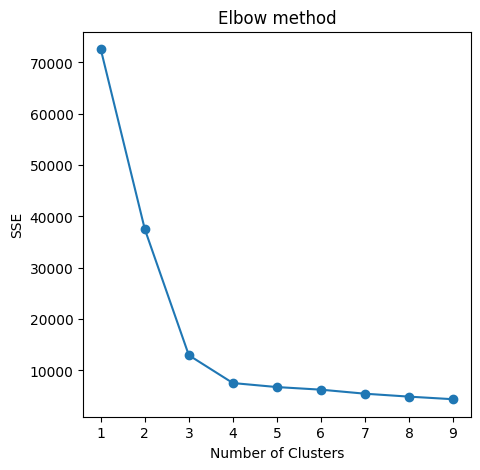
\includegraphics[width = 10cm, height = 7.5cm]{elbow-method.png}
			\end{figure}

\clearpage